\documentclass[12pt]{article}

\usepackage[margin = .8in]{geometry}
\usepackage{amsmath}
\usepackage{graphicx}
\usepackage{multicol, enumerate, tabularx}

\usepackage{adjustbox}

\usepackage{fancyhdr}
\pagestyle{fancy}

\lhead{Math F113X: Numbers and Society}
\rhead{Date: \hspace{1in}}

\usepackage{tikz}
\usetikzlibrary{calc,trees,positioning,arrows,fit,shapes,through, backgrounds}
\usetikzlibrary{patterns}

\usetikzlibrary{decorations.markings}
\usetikzlibrary{arrows}

\usepackage{pgfplots}

\usepackage{longtable}
\usepackage{tabularx}

\newcommand{\ds}{\displaystyle}
\newcommand{\ans}[1][1in]{\rule{#1}{.5pt}}

\newcommand{\points}[1]{(#1 points.)}		% Trying to be lazy.

\usepackage{array}
\newcolumntype{L}[1]{>{\raggedright\let\newline\\\arraybackslash\hspace{0pt}}m{#1}}
\newcolumntype{C}[1]{>{\centering\let\newline\\\arraybackslash\hspace{0pt}}m{#1}}
\newcolumntype{R}[1]{>{\raggedleft\let\newline\\\arraybackslash\hspace{0pt}}m{#1}}
\newcommand{\red}[1]{\textcolor{red}{#1}}

\newcommand{\be}{\begin{enumerate}}
\newcommand{\ee}{\end{enumerate}}

%\topmargin -1in
%\textheight 9.5in
%\oddsidemargin -0.3in
%\evensidemargin \oddsidemargin
%\pagestyle{empty}
%%\marginparwidth 0.5in
%\textwidth 7in
%\parindent 0in

%--------------------------------------------------------------------------------------------------------------------------------------------------------------------------
%						Document
%--------------------------------------------------------------------------------------------------------------------------------------------------------------------------


\begin{document}
%\pagestyle{fancy}
\begin{center}
{\Large  Worksheet 14 (Graph Theory 6): Hamiltonian Circuits}
\end{center}



\noindent \textbf{Group Names:} \hrulefill \\
%-------------------------------------------------------------------------------------------------------------
%						Assignment
%-----------------------------------------------------------------------------------------------------
\begin{enumerate}


\item Find a circuit in the following graphs that goes through every vertex exactly once: this is called a \emph{Hamiltonian circuit}. (It does not need to use every edge, of course!)

\begin{center}
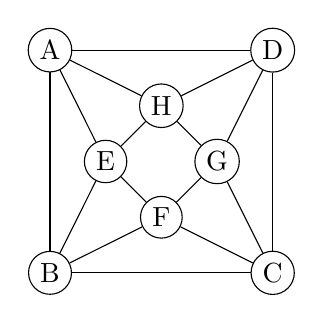
\begin{tikzpicture}[scale=2]

\tikzstyle{every node}=[circle, draw, fill=white,
                        inner sep=2pt]
%\draw (-1,2) node (A) {} -- (0,0) node (B) {} -- (1,2) node (C) {} -- (2,0) node (D) {} -- (3,2) node (F) {};
%\draw (A) -- (D);
%\draw (F) --(B);
%\foreach \i in {1,2,3,4}{ \node (\i) at (90*\i:1) {};}
%\foreach \i in {5,6,7,8}{\node let \n1 = int(\i-4) in  (\i) {};}

\node (1) at (-0.707, 0.707){A};
\node (2) at (-0.707, -0.707){B};
\node (3) at (0.707, -0.707){C};
\node (4) at (0.707, 0.707){D};
\node (5) at (-0.354, 0.){E};
\node (6) at (0., -0.354){F};
\node (7) at (0.354, 0.){G};
\node (8) at (0., 0.354){H};
%{1 \[UndirectedEdge] 2, 1 \[UndirectedEdge] 4, 1 \[UndirectedEdge] 5, 
% 1 \[UndirectedEdge] 8, 2 \[UndirectedEdge] 3, 2 \[UndirectedEdge] 5, 
% 2 \[UndirectedEdge] 6, 3 \[UndirectedEdge] 4, 3 \[UndirectedEdge] 6, 
% 3 \[UndirectedEdge] 7, 4 \[UndirectedEdge] 7, 4 \[UndirectedEdge] 8, 
% 5 \[UndirectedEdge] 6, 5 \[UndirectedEdge] 8, 6 \[UndirectedEdge] 7, 
% 7 \[UndirectedEdge] 8}
\foreach \i/\j in {1/2,1/4,1/5,1/8,2/3,2/5,2/6,3/4,3/6,3/7,4/7,4/8,5/6,5/8,6/7,7/8}{\draw (\i) -- (\j);}

\end{tikzpicture}
\end{center}

List the vertices in the circuit. \hrulefill

\item Find a Hamiltonian Circuit in the following graph.

\begin{center}
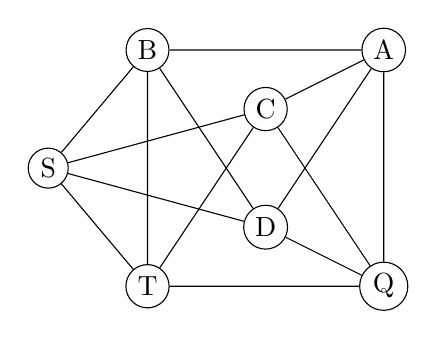
\begin{tikzpicture}[every node/.style={draw, circle, inner sep = 2pt}, scale = 1.5]
\node (1) at (1,1){A};
\node (2) at (1,-1) {Q};
\node (4) at (-1,-1) {T};
\node (6) at (-1,1) {B};
\node[left = of $(4)!.5!(6)$] (5)  {S};
\node (3) at (0, 1/2){C};  
\node (0) at (0, -1/2){D};  
\foreach \i in {0,1,2,3,4,5,6}{\draw let \n1 = {int(mod(\i+1, 7))}
 in (\i) -- (\n1);}
\foreach \i in {0,1,2,3,4,5,6}{\draw let \n1 = {int(mod(\i+2, 7))}
 in (\i) -- (\n1);}

\end{tikzpicture}
\end{center}

List the vertices in the circuit. \hrulefill

\item Find a Hamiltonian Path starting at vertex I. Then explain why you can't find a Hamiltonian circuit.

\begin{center}
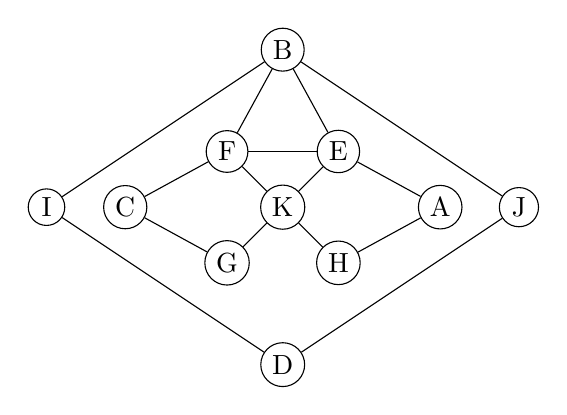
\begin{tikzpicture}[baseline=(current bounding box.center),scale = 1]
\tikzstyle{every node} = [draw, circle, inner sep = 2pt];
\node (A) at (0:2) {A};
\node (B) at (90:2) {B};
\node (C) at (180:2) {C};
\node (D) at (270:2) {D};
\node (O) at (0,0){K};
\node (E) at (45:1) {E};
\node (F) at (45+90:1){F};
\node (G) at (45+180:1){G};
\node (H) at (45+270:1){H};
\node[left of = C] (I) {I};
\node [right of = A] (J) {J};
\draw (B) -- (I) -- (D) -- (J)--(B);
\draw (A) -- (E) -- (B) -- (F) -- (C);
\draw (E) -- (O) -- (G) (F) --(O) --(H);
\draw (C) -- (G) (H) --(A);
\draw (E) -- (F) ;
\end{tikzpicture}
\end{center}

\vspace{1in}

\newpage

\item The following graph has (up to starting vertex and direction you go around the circuit) two Hamiltonian circuits. Highlight one on each copy of the graph and compute the total weight of the circuit. 

\bigskip

\begin{tabularx}{\linewidth}{X X}
\fbox{Circuit 1} & \fbox{Circuit 2}\\
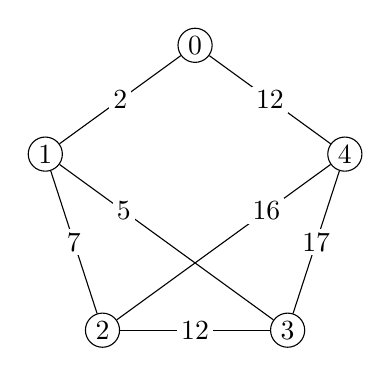
\begin{tikzpicture}[vtx/.style={draw, circle, inner sep =1.5 pt}, lbl/.style =  {inner sep =1.5 pt, fill = white}]
\foreach \i in {0,1,2,3,4}{\node[vtx] (\i) at (360*\i/5+90:2){\i};}
\foreach \i in {0,1,2,3,4}{\draw let \n1 = {int(mod(\i+1, 5))}, \n2 = {int(3*\i+2*\n1)}
 in (\i) -- node[lbl] {\n2} 
(\n1);}
\draw (1) -- node[pos = .3,lbl] {5} (3); 
    \draw (2) -- node[pos = .7,lbl] {16} (4); 
\end{tikzpicture}
&
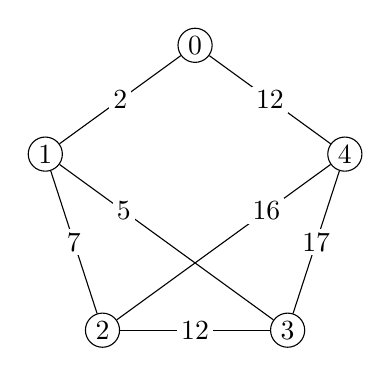
\begin{tikzpicture}[vtx/.style={draw, circle, inner sep =1.5 pt}, lbl/.style =  {inner sep =1.5 pt, fill = white}]
\foreach \i in {0,1,2,3,4}{\node[vtx] (\i) at (360*\i/5+90:2){\i};}
\foreach \i in {0,1,2,3,4}{\draw let \n1 = {int(mod(\i+1, 5))}, \n2 = {int(3*\i+2*\n1)}
 in (\i) -- node[lbl] {\n2} 
(\n1);}
\draw (1) -- node[pos = .3,lbl] {5} (3); 
    \draw (2) -- node[pos = .7,lbl] {16} (4); 
\end{tikzpicture}\\[16 pt]
Weight: \ans & Weight: \ans
\end{tabularx}

\vspace{1cm}

Which Hamiltonian circuit has the smallest weight? \ans

\item Use the Nearest Neighbor Algorithm starting at vertex 0 to find a Hamiltonian circuit. Highlight the circuit on the left-hand graph.

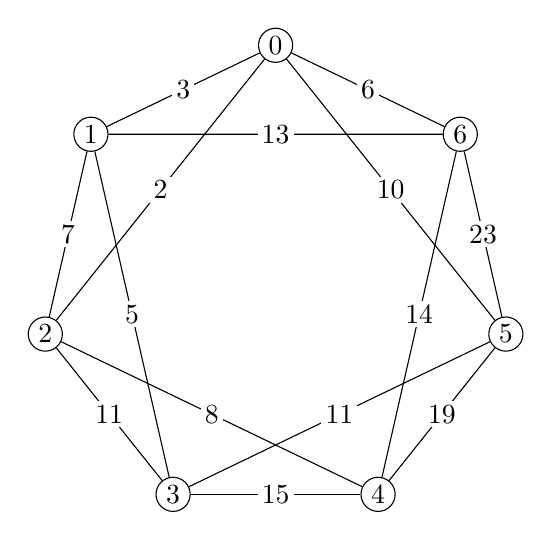
\begin{tikzpicture}[vtx/.style={draw, circle, inner sep =1.5 pt}, lbl/.style =  {inner sep =1.5 pt, fill = white}]
\foreach \i in {0,1,2,3,4,5,6}{\node[vtx] (\i) at (360*\i/7+90:3){\i};}
\foreach \i in {0,1,2,3,4,5,6}{\draw let \n1 = {int(mod(\i+1, 7))}, \n2 = {int(1*\i+3*\n1)}
 in (\i) -- node[lbl] {\n2} 
(\n1);}
\foreach \i in {0,1,2,3,4,5,6}{\draw let \n1 = {int(mod(\i+2, 7))}, \n2 = {int(2*\i+1*\n1)}
 in (\i) -- node[lbl] {\n2} 
(\n1);}
%\draw (1) -- node[pos = .3,lbl] {5} (3); 
%    \draw (2) -- node[pos = .7,lbl] {16} (4); 
\end{tikzpicture}
\hfill
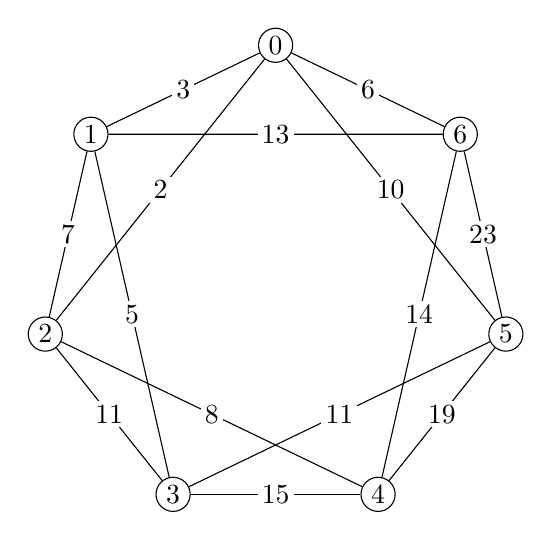
\begin{tikzpicture}[vtx/.style={draw, circle, inner sep =1.5 pt}, lbl/.style =  {inner sep =1.5 pt, fill = white}]
\foreach \i in {0,1,2,3,4,5,6}{\node[vtx] (\i) at (360*\i/7+90:3){\i};}
\foreach \i in {0,1,2,3,4,5,6}{\draw let \n1 = {int(mod(\i+1, 7))}, \n2 = {int(1*\i+3*\n1)}
 in (\i) -- node[lbl] {\n2} 
(\n1);}
\foreach \i in {0,1,2,3,4,5,6}{\draw let \n1 = {int(mod(\i+2, 7))}, \n2 = {int(2*\i+1*\n1)}
 in (\i) -- node[lbl] {\n2} 
(\n1);}
%\draw (1) -- node[pos = .3,lbl] {5} (3); 
%    \draw (2) -- node[pos = .7,lbl] {16} (4); 
\end{tikzpicture}
\bigskip

List the vertices of the circuit in order: \hrulefill

What is the weight of the circuit you found? \ans

Bonus: among all Hamiltonian circuits, the circuit with smallest weight has weight 61. Can you find it? Draw it on the second graph.



\end{enumerate}
\end{document}

%-------------------------------------------------------------------------------------------------------------------------------------------------------------------------------------------------------------------

%%% Local Variables:
%%% mode: latex
%%% TeX-master: t
%%% End:
